\documentclass[main.tex]{subfiles}
\graphicspath{{\subfix{../images/}}}
\begin{document}


Since $1/16$ of the iron supplement was used in the digestion,
\begin{equation}
    m_{\text{Fe in tablet}} = \frac{m_{1/16 \text{ tablet}}}{m_{\text{tablet}}}m_{\text{sample}}
    \label{eq:mass}
\end{equation}

The analysis was conducted on 50ml solutions that contained 2ml of a digested tablet sample that was dissolved in 100ml of water. Thus,
\begin{equation}
    C_{\text{sample}} = \frac{50 C_{\text{digested}}}{2}
    = 25C_{\text{digested}}
    \label{eq:test_digest}
\end{equation}

\begin{equation}
    m_{\text{sample}} = \frac{100\text{ ml}}{2\text{ ml}}  \times C_{\text{sample}} = 50 \times 0.002 \times 25 \times C_{\text{digested}}
    \label{eq:sample}
\end{equation}



Since standard linear calibration curve is in the form:
\begin{equation*}
    A = \frac{dy}{dx}C_{\text{digested}} + y_0
    \label{eq:cal_nosub}
\end{equation*}

Rearranging:
\begin{equation}
    C_{\text{digested}} = \frac{(A-y_0)}{\frac{dy}{dx}}
    \label{eq:conc_final_gen_eq}
\end{equation}
Substituting (\ref{eq:mass}), (\ref{eq:sample}), and (\ref{eq:test_digest}) to (\ref{eq:conc_final_gen_eq})
\begin{equation}
    m_{\text{Fe in tablet}} = 2.5 \times \frac{m_{1/16 \text{ tablet}}}{m_{\text{tablet}}} \times\frac{(A-y_0)}{\frac{dy}{dx}}
    \label{eq:mega}
\end{equation}



\subsection*{Sample}
\begin{table}[H]
    \centering
    \begin{tabular}{l|l}
\rowcolor[HTML]{FFC8F0} 
\textbf{} & \textbf{Mass} \\ \hline
\rowcolor[HTML]{FFE6F8} \textbf{Tablet}                   & 0.5769                                    \\
\rowcolor[HTML]{FFE6F8}\textbf{Theoretical 1/16 of mass} & 0.0361                                    \\
\rowcolor[HTML]{FFE6F8}\textbf{Actual 1/16 mass}         & 0.0364                                   
\end{tabular}

    \caption{Mass of tablet samples used}
    \label{tab:mass}
\end{table}
\begin{table}[H]
    \centering
    \begin{tabular}{l|l}
\rowcolor[HTML]{FFC8F0} 
\textbf{Sample} & \textbf{Absorbance} \\ \hline
\rowcolor[HTML]{FFE6F8} 
\textbf{a}      & 0.509               \\
\rowcolor[HTML]{FFE6F8} 
\textbf{b}      & 0.47                \\
\rowcolor[HTML]{FFE6F8} 
\textbf{c}      & 0.486              
\end{tabular}
    \caption{Absorbance at $\lambda = 508$ nm of digested iron supplement samples}
    \label{tab:sample_abs}
\end{table}

\subsection*{Calibration Curve}
As shown in Figure \ref{fig:colours}, visually, the quantity of orange light reflected - which is proportional to concentration - of the digested tablet samples are between 0.8 and 0.2ppm.
\begin{figure}[H]
    \centering
    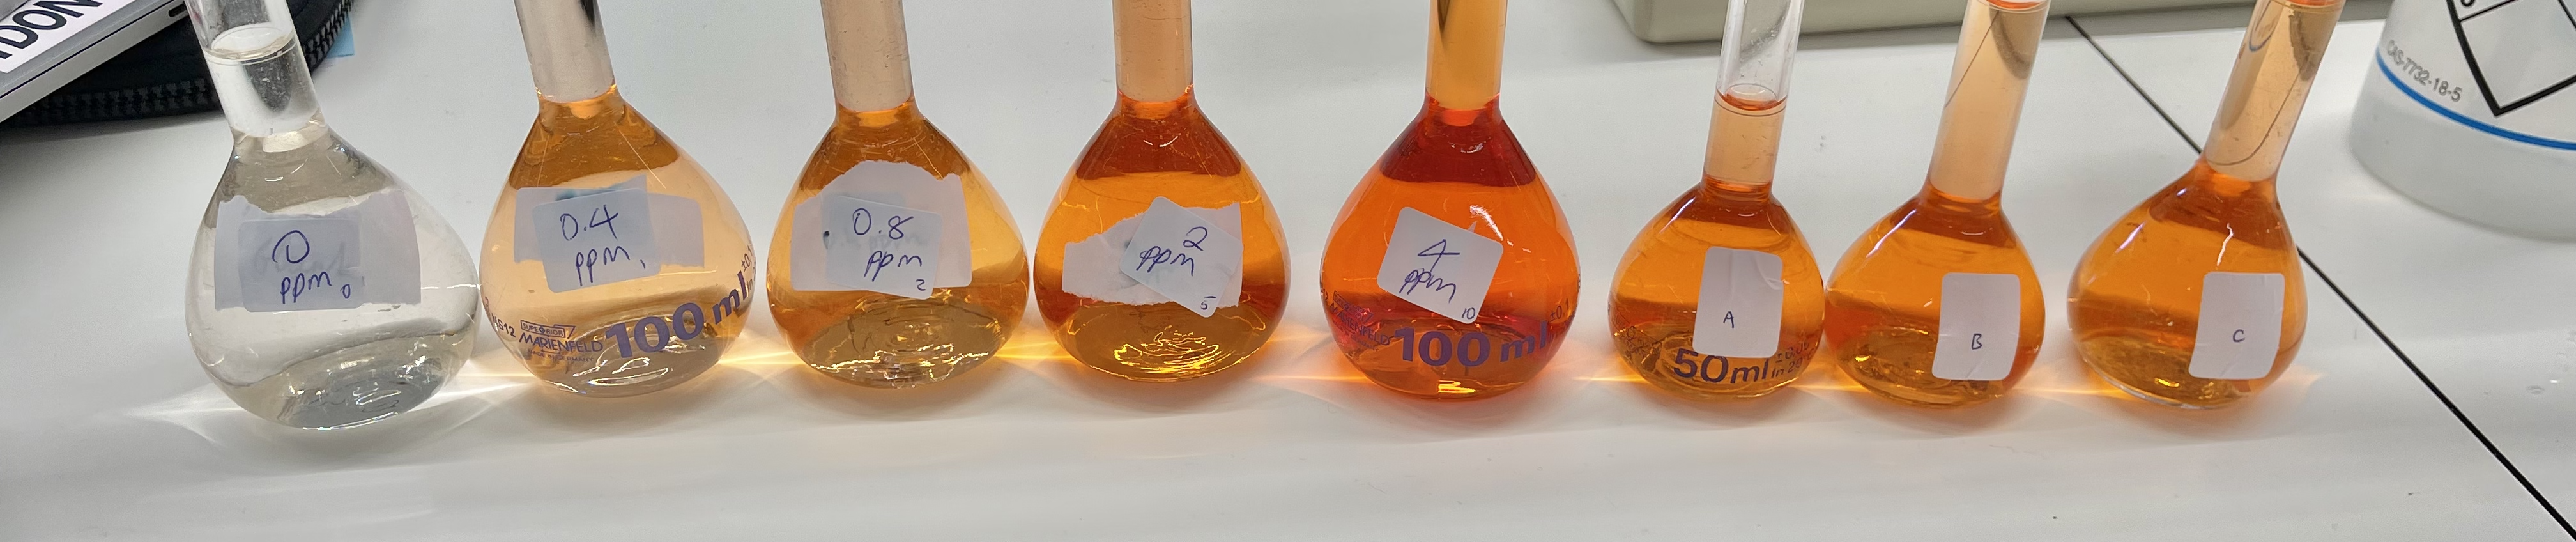
\includegraphics[width=\textwidth]{standards_colours.png}
    \caption{Standard solutions next to digested tablet samples.}
    \label{fig:colours}
\end{figure}

\begin{figure}[H]
    \centering
    \includegraphics[width=0.7\textwidth]{standard_curve.png}
    \caption{Standard calibration curve for absorbance at $\lambda=508$ nm}
    \label{fig:cal_curve}
\end{figure}
See Table \ref{tab:conc_table} in appendix.

\begin{table}[H]
    \centering
    \begin{tabular}{l|lll}
\rowcolor[HTML]{FFD7F4} 
\textbf{}                                  & \textbf{Coefficients} & \textbf{Upper 95\%} & \textbf{Lower 95\%} \\ \hline
\rowcolor[HTML]{FFE6F8} 
\cellcolor[HTML]{FFD7F4}\textbf{$y_0$} & -0.0077607            & -0.0303239          & 0.01480238          \\
\rowcolor[HTML]{FFE6F8} 
\cellcolor[HTML]{FFD7F4}\textbf{$\frac{dy}{dx}$}  & 0.21066718            & 0.1996047           & 0.22172966         
\end{tabular}
    \caption{95\% Confidence Interval}
    \label{tab:uncertainty}
\end{table}



Thus, the equation for the calibration curve is:
\begin{equation*}
    \mathcolorbox{Lavender}{A = 0.21066718C_{\text{digested}} -0.0077607}
\end{equation*}

\subsection*{Calculation of mass of iron in a supplement tablet}
By substituting values from Tables \ref{tab:mass} \ref{tab:uncertainty}, and \ref{tab:sample_abs} to Equation \ref{eq:mega},

\begin{table}[H]
    \centering
\begin{tabular}{l|ll}
\rowcolor[HTML]{FFC8F0} 
\textbf{Sample} & \textbf{Mass (mg)} & \textbf{Range (mg)}     \\ \hline
\rowcolor[HTML]{FFE6F8} 
\textbf{a}      & 97.1922855         & 88.3112496 - 107.05773  \\
\rowcolor[HTML]{FFE6F8} 
\textbf{b}      & 89.8571711         & 81.3420968 - 99.316089  \\
\rowcolor[HTML]{FFE6F8} 
\textbf{c}      & 92.8664488         & 84.2012364 - 102.492147
\end{tabular}
    \caption{Mass of iron in a tablet, $\sigma=3.6871967$ mg}
    \label{tab:all_mass}
\end{table}

Since the ranges overlap, the results are reproducible.




\end{document}